In questa sezione verranno presentati il protocollo ed i risultati della valutazione
dell'applicazione CookApp. Tale valutazione è finalizzata ad ottenere informazioni su
eventuali errori presenti nell'applicazione, ordinandoli per gravità e frequenza. Vengono
inoltre ottenute informazioni generali sull'impressione degli utenti nell'uso dell'applicazione,
rispetto alla sua usabilità.

\subsection{Il protocollo di test}
La modalità di test scelta è discount usability testing. Tale modalità risulta essere particolarmente
adatta, in quanto è sufficientemente snella da poter essere applicabile nel nostro contesto.
Verrà inoltre utilizzata la modalità ``thinking aloud'', nella quale gli utenti sono invitati a esplicitare
verbalmente le sensazioni e le problematiche che emergono durante l'utilizzo dell'applicazione.\\
Sono stati selezionati per i test 10 partecipanti fra conoscenti, amici e parenti in modo da coprire al meglio lo spettro
demografico individuato durante la fase di analisi etnografica, in particolare rispetto all'abilità culinaria e tecnologica.\\
Dopo il completamento di ciascun task si richiede ai partecipanti di valutare l'intuitività dell'operazione effettuata in una scala
Likert di valori compresi fra 1 e 5. Come descritto in precedenza, sono previsti valori nulli nel caso in cui non sia stato
possibile completare l'operazione. Oltre all'autovalutazione degli utenti, sarà compito dell'intervistatore annotare i suoi pensieri
ed eventuali errori e golfi fra l'intervistato e l'applicazione.
I task sono stati selezionati per esplorare in maniera esaustiva tutte le funzionalità principali offerti dall'applicazione.
Vengono di seguito elencati i task scelti:
\begin{enumerate}
 \item Cerca la ricetta ``spaghetti alla carbonara'' per nome;
 \item Cerca una ricetta selezionando solo la categoria ``primi'';
 \item Condividi la ricetta selezionata sul social network;
 \item Visualizza tutti i commenti associati ad una ricetta (spaghetti alla
	 carbonara);
 \item Lascia un commento sulla ricetta;
 \item Crea un menù;
 \item Trova una ricetta abbinabile al suddetto menù;
 \item Trova istruzioni video relative ad un passo della ricetta;
 \item Aggiungi ingredienti della ricetta selezionata alla lista della spesa;
 \item Trova un supermercato per fare la spesa;
 \item Simula un acquisto scannerizzando un prodotto;
 \item Simula l'acquisto delle arance;
 \item Chiedi aiuto per l'aglio;
 \item Modifica la dimensione del testo;
 \item Attiva la modalità ``non disturbare'';
 \item Aggiungi un utente allergico al menù, modifica la ricetta che crea problemi;
 \item Inizia a preparare il menù e chiedi aiuto per un passo della ricetta;
 \item Aggiungi gli spaghetti ai preferiti;
 \item Trova i preferiti.
\end{enumerate}

\subsection{Risultati dei test}
\begin{quote}
	\textbf{1. Cerca la ricetta ``spaghetti alla carbonara'' per nome}
\end{quote}
Soddisfazione attesa media: 5\\
Soddisfazione riscontrata media: 5\\
Il task è risultato molto semplice ed è stato completato con successo da tutti
i partecipanti.

\begin{quote}
	\textbf{2. Cerca una ricetta selezionando solo la categoria ``primi''}
\end{quote}
Soddisfazione attesa media: 4,25\\
Soddisfazione riscontrata media: 4,75\\
Non sono stati riscontrati particolari errori o golfi impedenti il completamento
del task.

\begin{quote}
	\textbf{3. Condividi la ricetta selezionata sul social network}
\end{quote}
Soddisfazione attesa media: 3,75\\
Soddisfazione riscontrata media: 3,75\\
Il task è stato inizialmente ritardato da un pulsante il quale significato è
risultato di difficile comprensione.

\begin{quote}
	\textbf{4. Visualizza tutti i commenti associati ad una ricetta (spaghetti
	 alla carbonara)}
\end{quote}
Soddisfazione attesa media: 4,5\\
Soddisfazione riscontrata media: 5\\
Il task è risultato molto semplice.

\begin{quote}
	\textbf{5. Lascia un commento sulla ricetta}
\end{quote}
Soddisfazione attesa media: 4\\
Soddisfazione riscontrata media: 5\\
Il task non ha creato problemi agli utenti ed è stato completato con successo.

\begin{quote}
	\textbf{6. Crea un menù}
\end{quote}
Soddisfazione attesa media: 3\\
Soddisfazione riscontrata media: 4\\
Il task viene completato in tempi molto brevi, data anche l'immediatezza del
pulsante ``Aggiungi nuovo menù''.

\begin{quote}
	\textbf{7. Trova una ricetta abbinabile al suddetto menù}
\end{quote}
Soddisfazione attesa media: 2,75\\
Soddisfazione riscontrata media: 3,25\\
Gli utenti hanno riscontrato alcune difficoltà nel comprendere che il task
richiedesse l'aggiunta di un piatto.

\begin{quote}
	\textbf{8. Trova istruzioni video relative ad un passo della ricetta}
\end{quote}
Soddisfazione attesa media: 4\\
Soddisfazione riscontrata media: 4,75\\
Non sono stati evidenziati problemi gravi durante l'analisi.

\begin{quote}
	\textbf{9. Aggiungi ingredienti della ricetta selezionata alla lista della
	spesa}
\end{quote}
Soddisfazione attesa media: 3,25\\
Soddisfazione riscontrata media: 5\\
L'interfaccia per l'aggiunta degli ingredienti risulta immediata non impedendo in alcun modo la riuscita del task.

\begin{quote}
	\textbf{10. Trova un supermercato per fare la spesa}
\end{quote}
Soddisfazione attesa media: 3\\
Soddisfazione riscontrata media: 4\\
L'interfaccia risulta leggermente meno immediata, il pulsante di navigazione ha
richiesto agli utenti qualche secondo per essere individuato, il che comunque non
ha impedito la buona riuscita del task.

\begin{quote}
	\textbf{11. Simula un acquisto scannerizzando un prodotto}
\end{quote}
Soddisfazione attesa media: 3,25\\
Soddisfazione riscontrata media: 4,75\\
Il task è risultato semplice dato il pulsante ben visibile.

\begin{quote}
	\textbf{12. Simula l'acquisto delle arance}
\end{quote}
Soddisfazione attesa media: 4,25\\
Soddisfazione riscontrata media: 5\\
Il task è immediato, dato anche l'utilizzo di checkbox.

\begin{quote}
	\textbf{13. Chiedi aiuto per l'aglio}
\end{quote}
Soddisfazione attesa media: 3\\
Soddisfazione riscontrata media: 4\\
Il task è stato completato con modalità differenti.  Nel caso della richiesta
d'aiuto dalla lista della spesa, il pulsante di aiuto e condivisione non è
risultato molto chiaro.

\begin{quote}
	\textbf{14. Modifica la dimensione del testo}
\end{quote}
Soddisfazione attesa media: 3,25\\
Soddisfazione riscontrata media: 5\\
Le impostazioni risultano sufficientemente chiare e facilmente raggiungibili.

\begin{quote}
	\textbf{15. Attiva la modalità ``non disturbare''}
\end{quote}
Soddisfazione attesa media: 4\\
Soddisfazione riscontrata media: 5\\
Una volta raggiunte le impostazioni il task risulta molto semplice.  È però
stato richiesto di descrivere meglio la funzionalità in esame.

\begin{quote}
	\textbf{16. Aggiungi un utente allergico al menù, modifica la ricetta che
	crea problemi}
\end{quote}
Soddisfazione attesa media: 3,25\\
Soddisfazione riscontrata media: 4\\
variando task è stato completato anche se l'interfaccia di modifica non invitava a
risolvere il problema variando la ricetta.

\begin{quote}
	\textbf{17. Inizia a preparare il menù e chiedi aiuto per un passo della
	ricetta}
\end{quote}
Soddisfazione attesa media: 3,25\\
Soddisfazione riscontrata media: 3,25\\
Gli utenti hanno riscontrato difficoltà nel comprendere come iniziare a
preparare la ricetta.  Inoltre il pulsante per richiedere aiuto non era
consistente con il resto dell'applicazione, risultando di difficile
comprensione.

\begin{quote}
	\textbf{18. Aggiungi gli spaghetti ai preferiti}
\end{quote}
Soddisfazione attesa media: 4,75\\
Soddisfazione riscontrata media: 5\\
Il task risulta immediato grazie all'utilizzo di un simbolo universale quale il
cuore.

\begin{quote}
	\textbf{19. Trova i preferiti}
\end{quote}
Soddisfazione attesa media: 4,5\\
Soddisfazione riscontrata media: 5\\
I preferiti sono facilmente raggiungibili dal menù laterale, che rende semplice
la navigazione dell'applicazione.

\subsection{Modifiche effettuate al sistema}
Date le precedenti segnalazioni da parte degli utenti, sono state effettuate
alcune modifiche all'interfaccia per migliorarne l'usabilità generale.

\begin{quote}
	\textbf{Dimensione del testo}
\end{quote}
In tutti i task precedenti si è riscontrata una generale difficoltà nella
lettura del testo, il quale risultava troppo piccolo.  Si è quindi provveduto ad
aumentare la dimensione del testo in ogni schermata.  Per mantenere il tutto
fruibile e coerente sono stati modificate anche le dimensioni dei pulsanti per
aggiungere le ricette ai preferiti.

\begin{figure}[H]
	\begin{minipage}{.49\textwidth}
		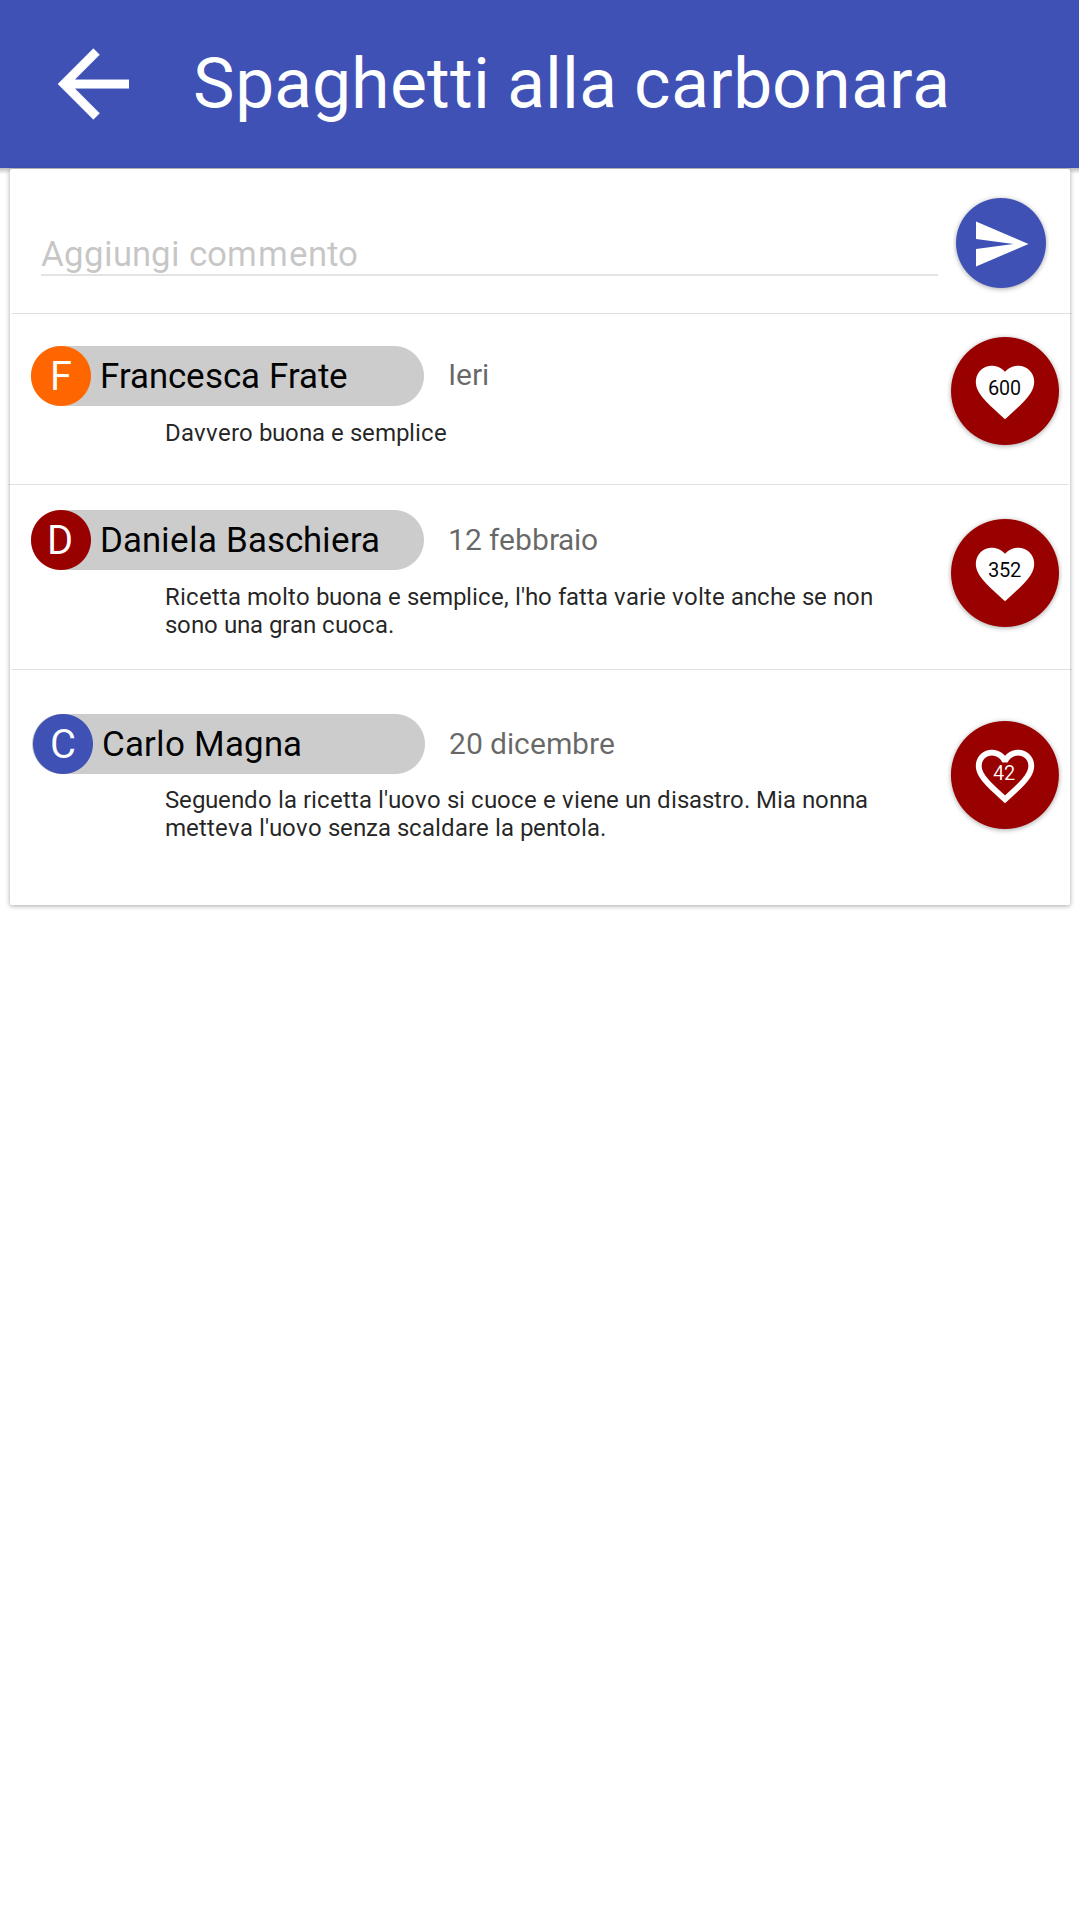
\includegraphics[width=\textwidth]{img/modifiche/commenti_old.png}
	\end{minipage}
	\begin{minipage}{.49\textwidth}
		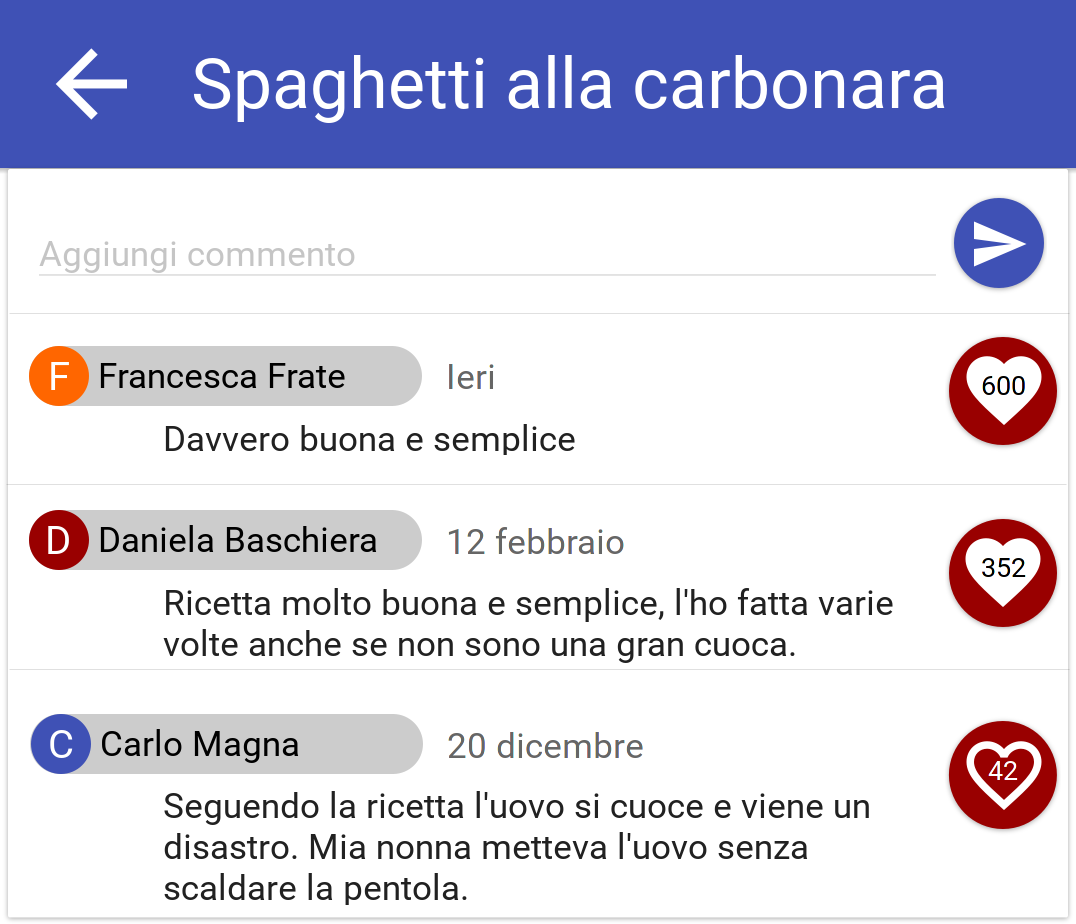
\includegraphics[width=\textwidth]{img/modifiche/commenti_new.png}
	\end{minipage}
\end{figure}

\begin{quote}
	\textbf{Inviti modifiche ricetta}
\end{quote}

L'interfaccia per la modifica delle ricette, in caso di un utente intollerante
ad un certo alimento non presentavano inviti per indurre al click su
di essi.  Sono quindi state modificate le card relative aggiungendo un pulsante
specifico per ogni azione.
\begin{figure}[H]
	\begin{minipage}{.49\textwidth}
		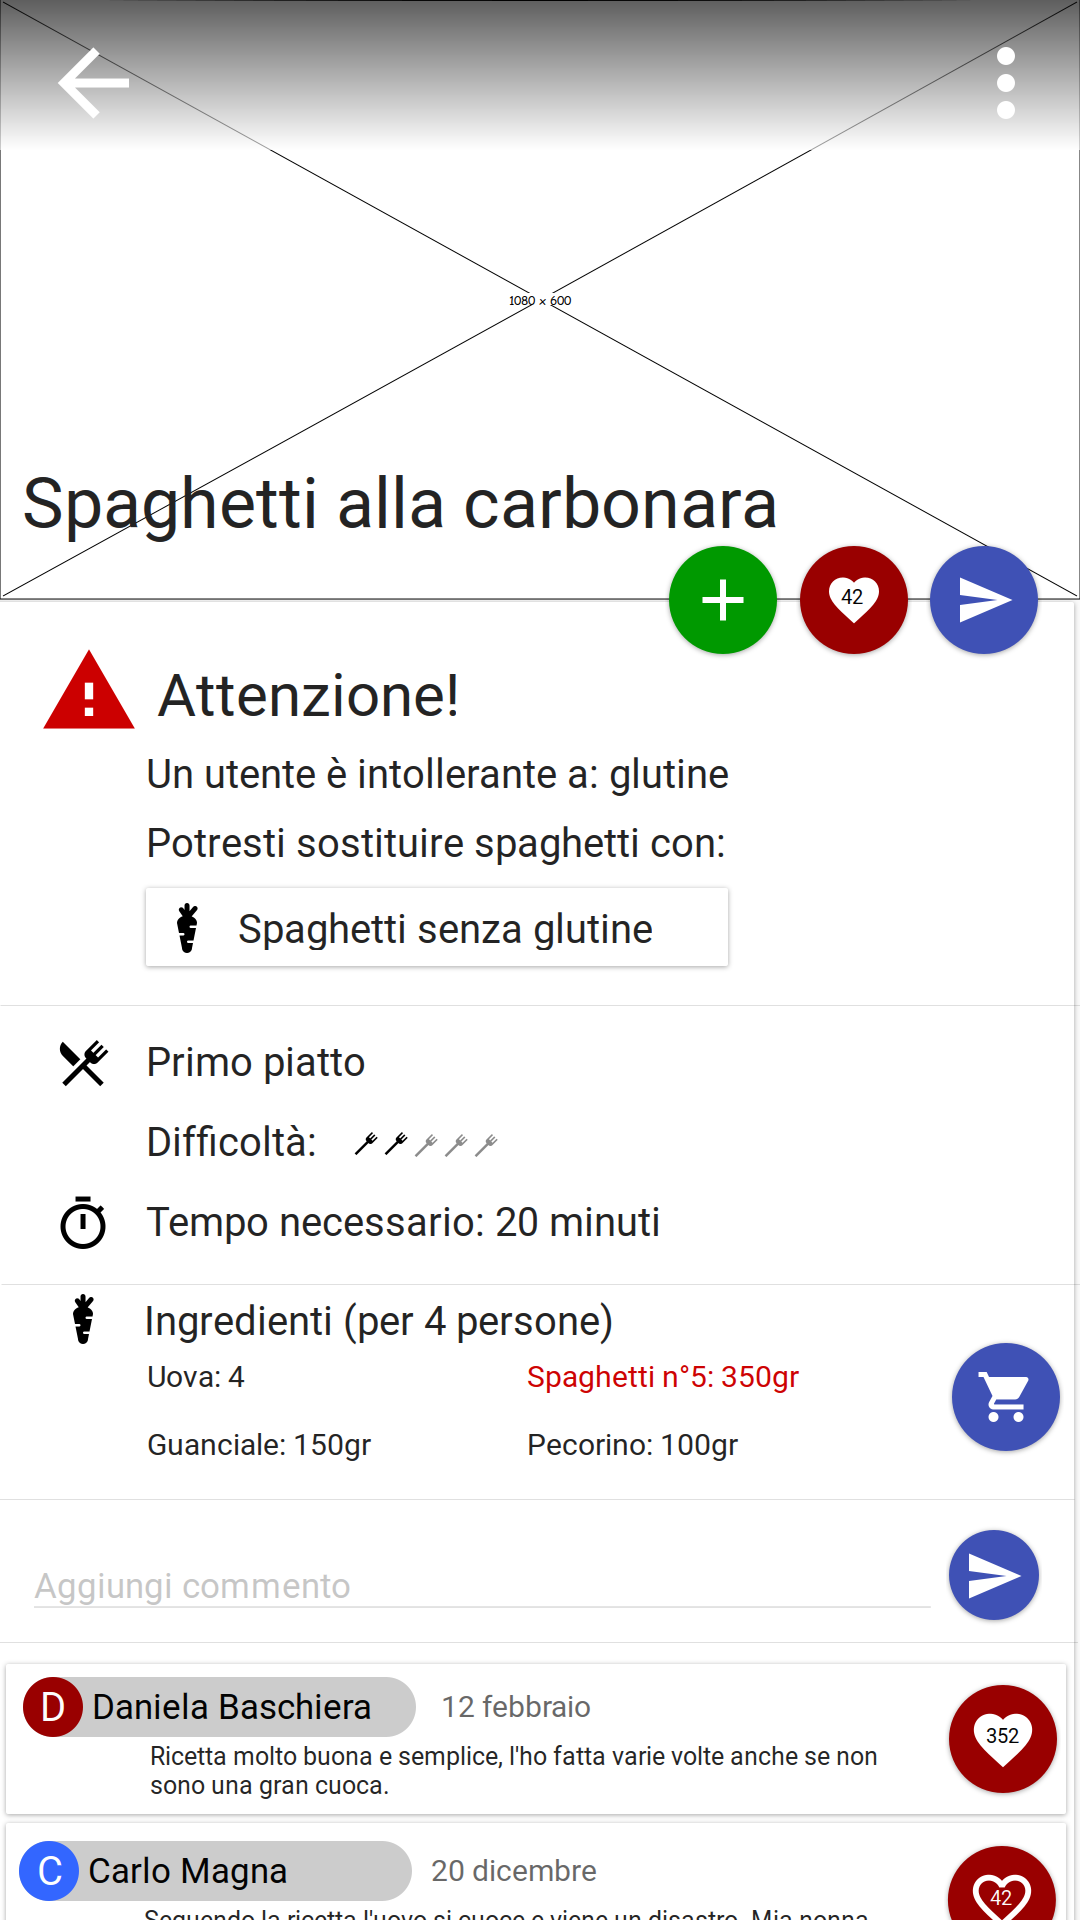
\includegraphics[width=\textwidth]{img/modifiche/cambia_ingrediente_old.png}
	\end{minipage}
	\begin{minipage}{.49\textwidth}
		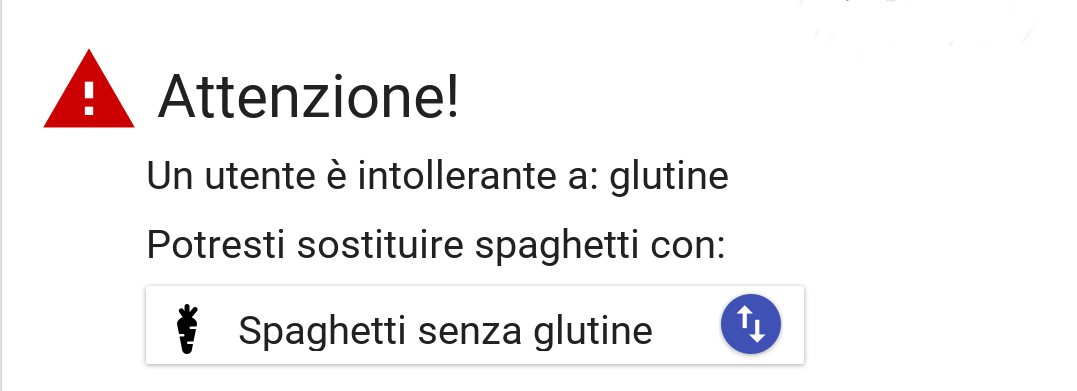
\includegraphics[width=\textwidth]{img/modifiche/cambia_ingrediente_new.png}
	\end{minipage}
\end{figure}

I simboli associati a questi pulsanti sono stati selezionati tra:
\begin{itemize}
	\item Swap Verticale per sostituire l'ingrediente con uno compatibile;
	\item Swap orizzontale per sotituire la ricetta con una compatibile;
	\item Cestino dell'immondizia per rimuovere la ricetta dal menù.
\end{itemize}
\begin{figure}[H]
	\centering
		
\includegraphics[width=.12\textwidth]{img/icons/swapvert}
		
\includegraphics[width=.12\textwidth]{img/icons/swaphor}
		
\includegraphics[width=.12\textwidth]{img/icons/delete}
	\caption{Simboli relativi alle varie operazioni}
\end{figure}

\begin{quote}
	\textbf{Modifica del pulsante ``inizia a cucinare una ricetta''}
\end{quote}
È stata segnalata dai partecipanti la bassa chiarezza del pulsante inizia a
cucinare (associato all'icona di invio del pacchetto di icone di material
design).  Per risolvere questo inconveniente e migliorare l'interfaccia, è stato
modificato il suddetto pulsante associandolo ad un'icona raffigurante una
pentola\footnote{Tale icona non è presente nel pacchetto di icone ufficiale di
material design, è bensì un'icona introdotta dalla comunità.}, per richiamare il concetto di cucina.
\begin{figure}[H]
	\begin{minipage}{.49\textwidth}
		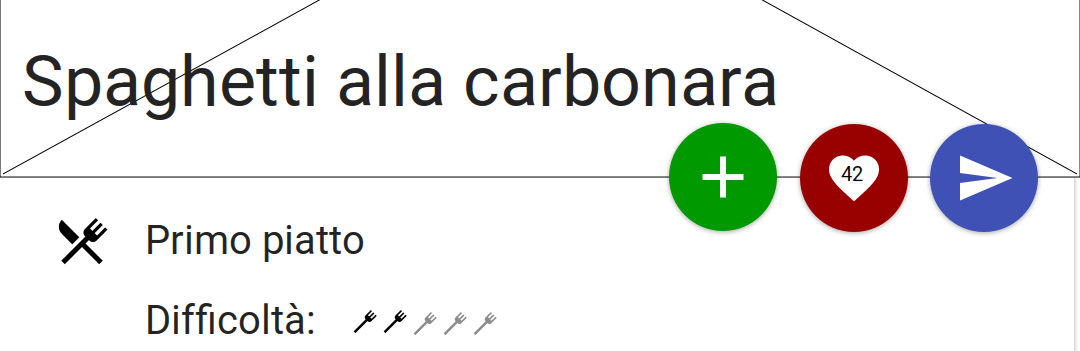
\includegraphics[width=\textwidth]{img/modifiche/presentazione_ricetta_old2.png}
	\end{minipage}
	\begin{minipage}{.49\textwidth}
		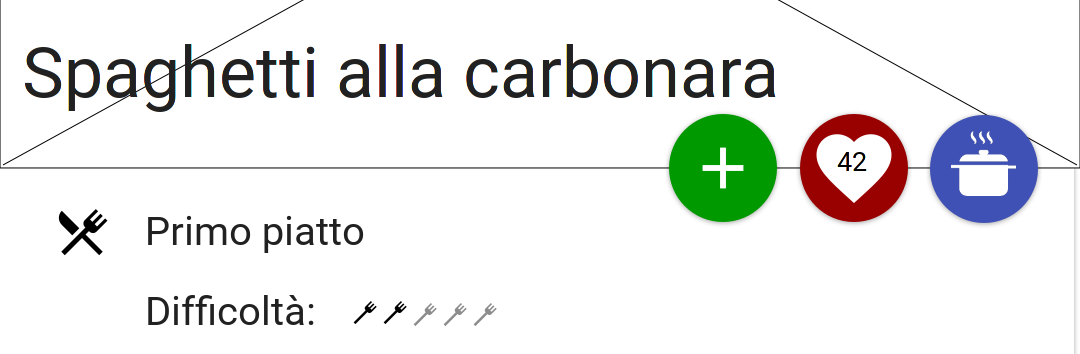
\includegraphics[width=\textwidth]{img/modifiche/presentazione_ricetta_new.png}
	\end{minipage}
\end{figure}

\begin{quote}
	\textbf{Pulsante d'aiuto}
\end{quote}
Inizialmente il pulsante di aiuto condivideva il simbolo con il simbolo di
condivisione sul social network, ricalcando questa funzione.  Questa scelta
progettuale però, non si è rivelata comprensibile e coerente con l'interfaccia
dell'intera applicazione.  Si è quindi provveduto a modificare la suddetta icona
con un'icona più esplicativa e ricalcante il concetto di aiuto.
\begin{figure}[H]
	\begin{minipage}{.49\textwidth}
		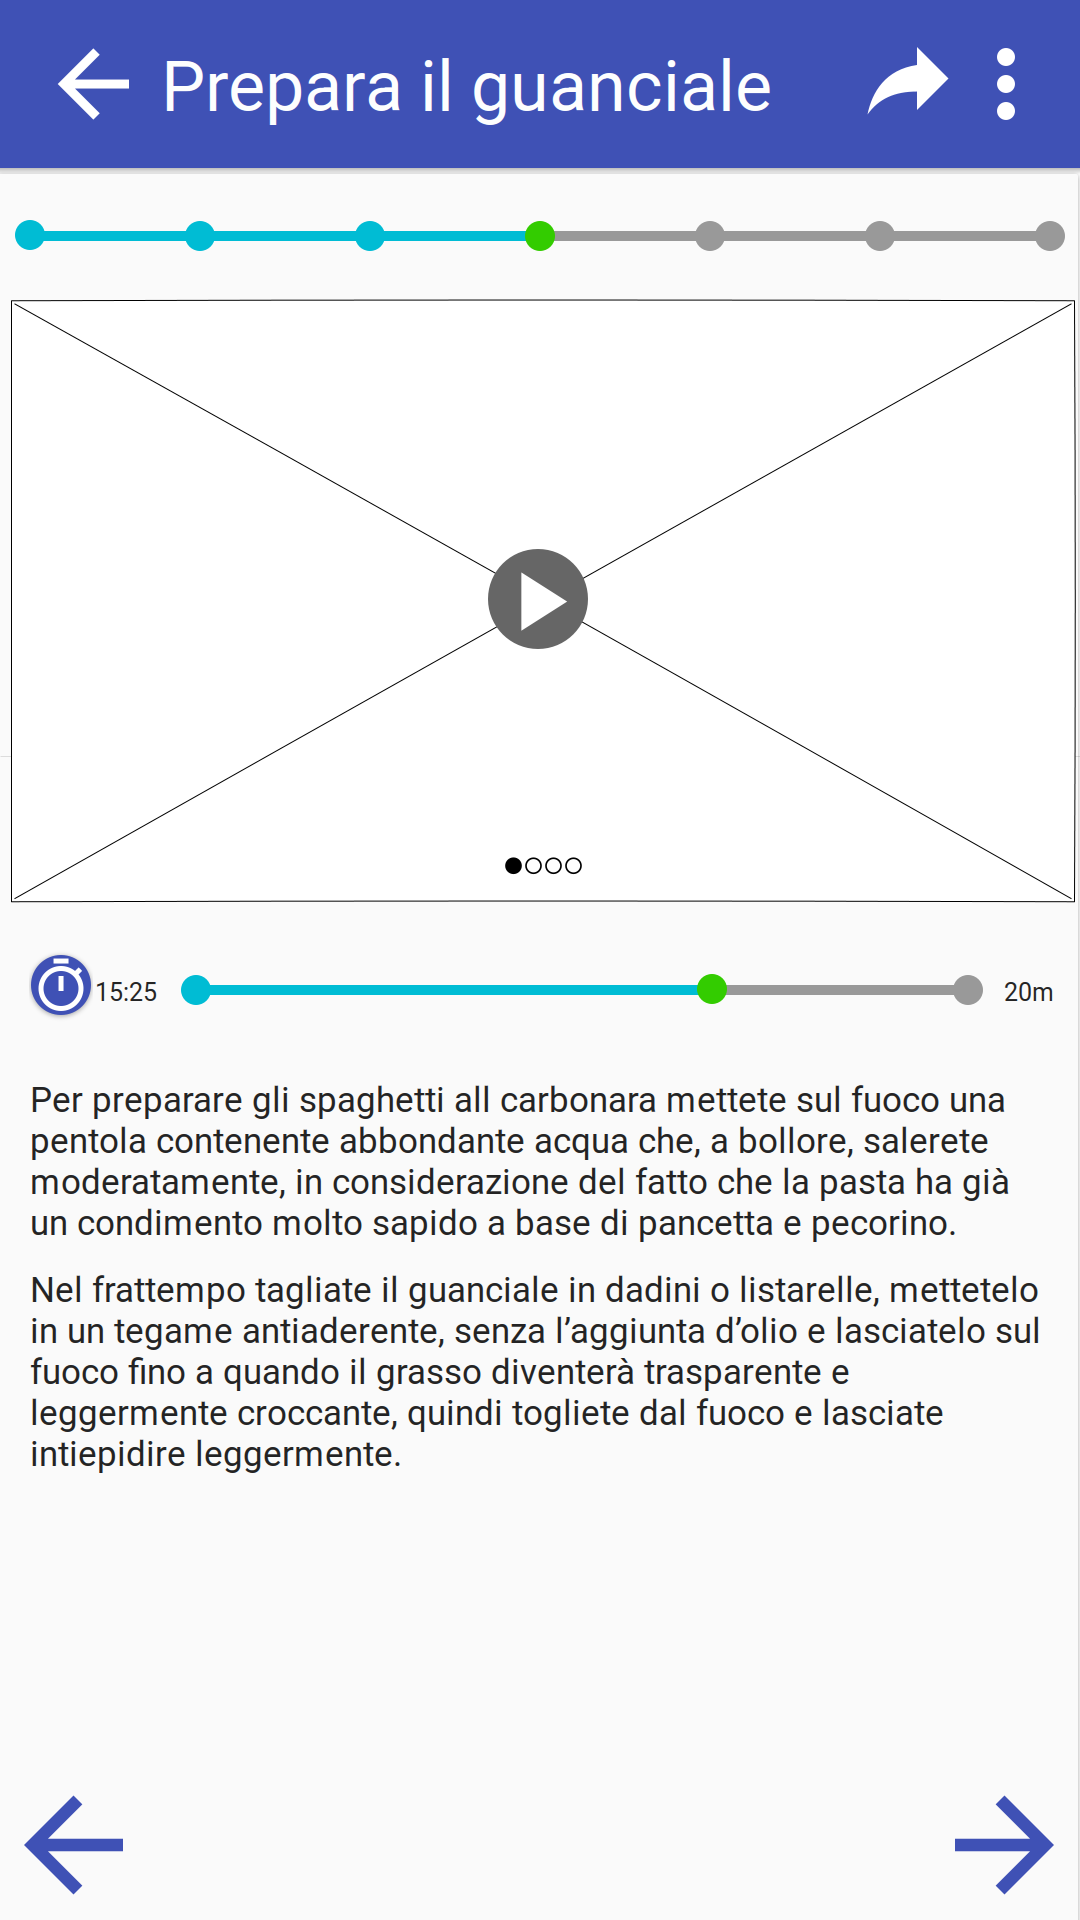
\includegraphics[width=\textwidth]{img/modifiche/condividi_passo_old.png}
	\end{minipage}
	\begin{minipage}{.49\textwidth}
		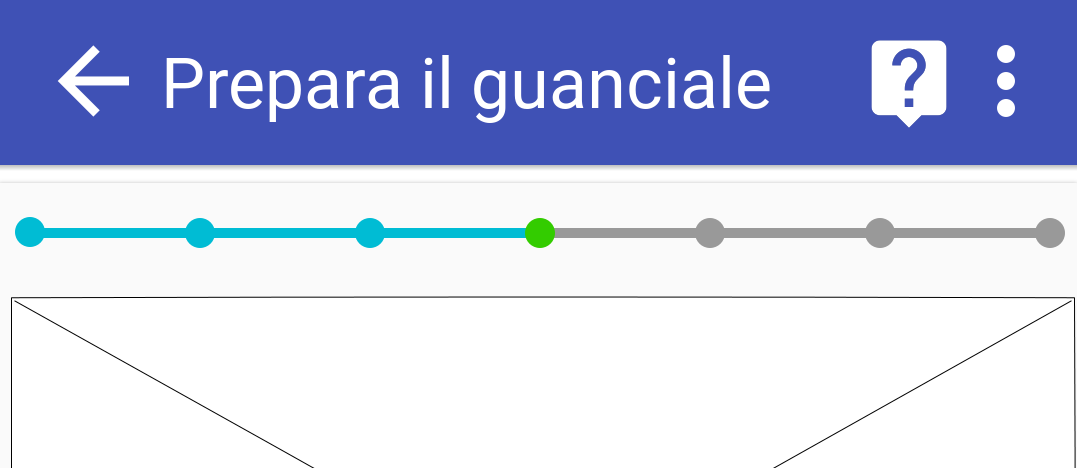
\includegraphics[width=\textwidth]{img/modifiche/condividi_passo_new.png}
	\end{minipage}
\end{figure}

\begin{quote}
	\textbf{Descrizione modalità non disturbare}
\end{quote}
La modalità non disturbare presentava un grande controllo e facilità di
utilizzo, tale modalità non era però documentata.  Il che contribuiva a rendere
l'applicazione meno usabile e lasciava all'utente il compito di comprendere da
solo in cosa sussistesse la suddetta modalità.  È stata quindi aggiunta una
piccola sezione informativa nell'area sottostante all'impostazione.
\begin{figure}[H]
	\begin{minipage}{.49\textwidth}
		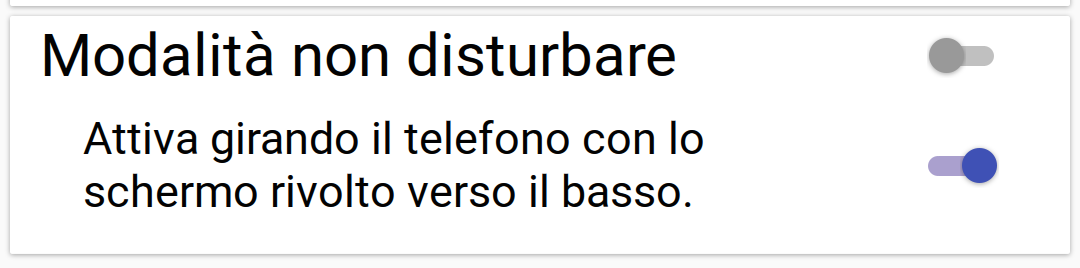
\includegraphics[width=\textwidth]{img/modifiche/non_disturbare_old.png}
	\end{minipage}
	\begin{minipage}{.49\textwidth}
		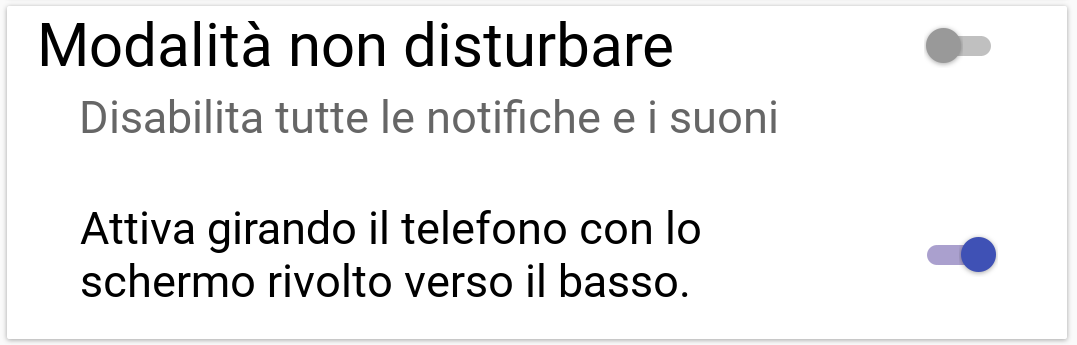
\includegraphics[width=\textwidth]{img/modifiche/non_disturbare_new.png}
	\end{minipage}
\end{figure}
